%% CLIP-RDS: SIGSPATIAL 2026 short paper draft (ACM sigconf).
%% Built from the SIGSPATIAL 2026 acmart template (template/main.tex).
%% Items to fix before submission are marked CHECK or TODO in comments.
%%
%% Table 2: validation year 2024 (also used for early stopping).
%% Table 3: test year 2025, scored once with the final models on 2026-11-13
%% (figures/scores_test.csv, scores_test_seeds.csv). Do not re-score.

\documentclass[sigconf]{acmart}

\AtBeginDocument{%
  \providecommand\BibTeX{{%
    Bib\TeX}}}

%% CHECK: replace with the rights information received after acceptance.
\setcopyright{none}
\settopmatter{printacmref=false}
\renewcommand\footnotetextcopyrightpermission[1]{}
\acmConference[SIGSPATIAL '26]{The 34th ACM International Conference on
  Advances in Geographic Information Systems}{2026}{CHECK location}
%% CHECK: the conference edition, dates and location above

\usepackage{booktabs}
\usepackage{multirow}

\begin{document}

\title[Does CLIP Help Rainfall Downscaling?]{Does Vision--Language
  Pretraining Help Rainfall Downscaling? A Controlled Study with CLIP
  over Thailand}

%% CHECK: Prof. Vateekul's e-mail, and both authors' department names
\author{Sudarshan Tamang}
\email{tamangsudarshan213@gmail.com}
\affiliation{%
  \institution{Chulalongkorn University}
  \city{Bangkok}
  \country{Thailand}}

\author{Peerapon Vateekul}
\email{[advisor e-mail]}
\affiliation{%
  \institution{Chulalongkorn University}
  \city{Bangkok}
  \country{Thailand}}

\renewcommand{\shortauthors}{Tamang et al.}

\begin{abstract}
  Deep-learning downscaling models trained with pixel-wise losses produce
  smooth fields and underestimate heavy rain. Vision--language models such
  as CLIP have been proposed as a source of high-level supervision for
  precipitation tasks. We test this idea for statistical downscaling of
  ERA5 (0.25\textdegree) to CHIRPS (0.05\textdegree) over Thailand in the
  monsoon season, using a residual U-Net. We use frozen CLIP in two ways:
  (i) as a training loss that aligns predicted rain maps with sentences
  describing observed heavy rain, and (ii) as an input, by feeding CLIP
  patch features of the ERA5 rain map into the U-Net bottleneck. Neither
  CLIP loss fixed the underestimation; quantile mapping remained far more
  effective. Diagnostics show why: CLIP chose the right sentence for only
  22\% of rain-map crops (chance 25\%), and its features added no
  significant information beyond simple ERA5 statistics; RemoteCLIP and
  SigLIP did no better. The input variant, combined with quantile mapping,
  gave a small gain over U-Net with quantile mapping on the 2024 validation
  year (CSI at 20\,mm: 0.282 vs.\ 0.275, three seeds). However, a randomly
  initialised network of the same architecture recovered most of this gain
  (0.280), and on the held-out 2025 test year it matched CLIP (0.273
  vs.\ 0.271; U-Net with quantile mapping: 0.263). The benefit therefore
  comes from the extra input path, not from vision--language pretraining. We argue that such random-weight
  controls should accompany claims that foundation models help geospatial
  downscaling.
\end{abstract}

%% CHECK: regenerate with the ACM CCS tool (https://dl.acm.org/ccs) if needed
\begin{CCSXML}
<ccs2012>
 <concept>
  <concept_id>10010147.10010257.10010293.10010294</concept_id>
  <concept_desc>Computing methodologies~Neural networks</concept_desc>
  <concept_significance>500</concept_significance>
 </concept>
 <concept>
  <concept_id>10010405.10010432.10010437</concept_id>
  <concept_desc>Applied computing~Earth and atmospheric sciences</concept_desc>
  <concept_significance>500</concept_significance>
 </concept>
</ccs2012>
\end{CCSXML}

\ccsdesc[500]{Computing methodologies~Neural networks}
\ccsdesc[500]{Applied computing~Earth and atmospheric sciences}

\keywords{precipitation downscaling, vision--language models, CLIP, U-Net,
  heavy rainfall, quantile mapping, ablation}

\maketitle

%% ---------------------------------------------------------------------
\section{Introduction}

Global reanalyses such as ERA5~\cite{hersbach2020era5} describe the
atmosphere at about 25\,km, too coarse for flood and urban-drainage
applications that need rainfall at a few kilometres. Statistical
downscaling learns a mapping from coarse fields to fine observations, and
convolutional networks have become a standard tool for
it~\cite{vandal2017deepsd,banomedina2020,rampal2024review,harder2023constrained}. Networks trained with a
pixel-wise loss, however, learn the conditional mean: when the position of
a storm is uncertain, they spread its rain out and flatten its peak. This
``double penalty'' leads to systematic underestimation of heavy rain,
exactly the events that matter most. Common remedies are bias correction
after training, such as quantile mapping (QM)~\cite{gudmundsson2012qm},
losses based on spatial verification
scores~\cite{lagerquist2022spatial}, and generative models such as
CorrDiff~\cite{mardani2025corrdiff} and related
approaches~\cite{price2022increasing,hess2025consistency,lopezgomez2025dynamical}.

At the same time, large pretrained models are spreading through the
geosciences: weather and climate models trained on
reanalysis~\cite{lam2023graphcast,price2025gencast,bodnar2025aurora,nguyen2023climax,schmude2024prithviwxc,rasp2024weatherbench2},
and vision--language models adapted to satellite
imagery~\cite{liu2024remoteclip,zhang2024rs5m,wang2024skyscript,kuckreja2024geochat,klemmer2025satclip}.
A recent line of work uses CLIP~\cite{radford2021clip}, a model trained
on 400 million image--caption pairs, as a source of high-level supervision
for rain-related vision tasks. For radar precipitation nowcasting,
Clip4Rain~\cite{li2026clip4rain} adds two CLIP-based terms to a
pixel-wise loss: a multi-scale consistency term on encoder and decoder
features, and a multi-level regional alignment (MRA) loss. MRA crops the
predicted and observed frames into nested regions and asks that both have
the same CLIP similarity to text prompts such as ``there are
[$n$] rain pixels in the image'', an idea taken from crowd
counting~\cite{liang2023crowdclip}. Clip4Rain reports a 37\% higher CSI than
the next-best method at the heaviest threshold on the KNMI radar dataset. If CLIP's notion of
``a lot of rain'' transferred to rain maps, such a loss could reward
realistic heavy-rain structure that a pixel-wise loss cannot. Whether this
carries over to downscaling, a different task with daily rather than
5-minute data, and whether the gains come from pretraining at all, has not
been tested.

We test this hypothesis carefully. Our contributions are:
\begin{itemize}
  \item A downscaling study over Thailand (ERA5 to CHIRPS, 5$\times$
  refinement) comparing a residual U-Net, QM, a heavy-rain count loss and
  two CLIP losses adapted from MRA.
  \item Diagnostics of whether CLIP, RemoteCLIP~\cite{liu2024remoteclip}
  and SigLIP~\cite{zhai2023siglip} can read rain maps at all.
  \item A scale-consistent way to feed CLIP patch features into a U-Net,
  evaluated over three seeds against a random-weight control of the same
  architecture.
\end{itemize}
The control changes the conclusion: the small gain from CLIP features is
mostly reproduced without any pretraining.

%% ---------------------------------------------------------------------
\section{Data and Experimental Setup}

\textbf{Region and period.} Thailand and its surroundings
(5--21\textdegree N, 97--106\textdegree E), May to October (the monsoon
season). We train on 2022--2023 (366 days), validate on 2024 (183 days)
and test on 2025 (183 days). The test year was scored only once, with
the final models, after all design choices had been fixed. Bangkok
(13.5--14.0\textdegree N, 100.3--100.9\textdegree E) is also scored
separately, as an urban area where flooding matters most.

\textbf{Inputs.} Daily ERA5~\cite{hersbach2020era5} at 0.25\textdegree:
total precipitation (summed over 00--24\,UTC), total column water vapour,
and the zonal and meridional wind at 850\,hPa. All four are interpolated
bilinearly to the target grid and normalised with training statistics;
rain is used as $\log(1+r)$.

\textbf{Target.} CHIRPS v2.0~\cite{funk2015chirps} daily rainfall at
0.05\textdegree{} ($320\times180$ cells), which covers land only and
performs well against gauges over Thailand~\cite{kaprom2025thailand}. All
scores are computed over land cells.

\textbf{Metrics.} Mean absolute error (MAE), mean bias (prediction minus
observation), and Pearson correlation over all land cell-days. For heavy
rain, we use the critical success index~\cite{schaefer1990csi}
$\mathrm{CSI} = H/(H+M+F)$ at 20 and 50\,mm/day, where $H$, $M$ and $F$
count hits, misses and false alarms.

%% ---------------------------------------------------------------------
\section{Methods}

\begin{figure*}
  \centering
  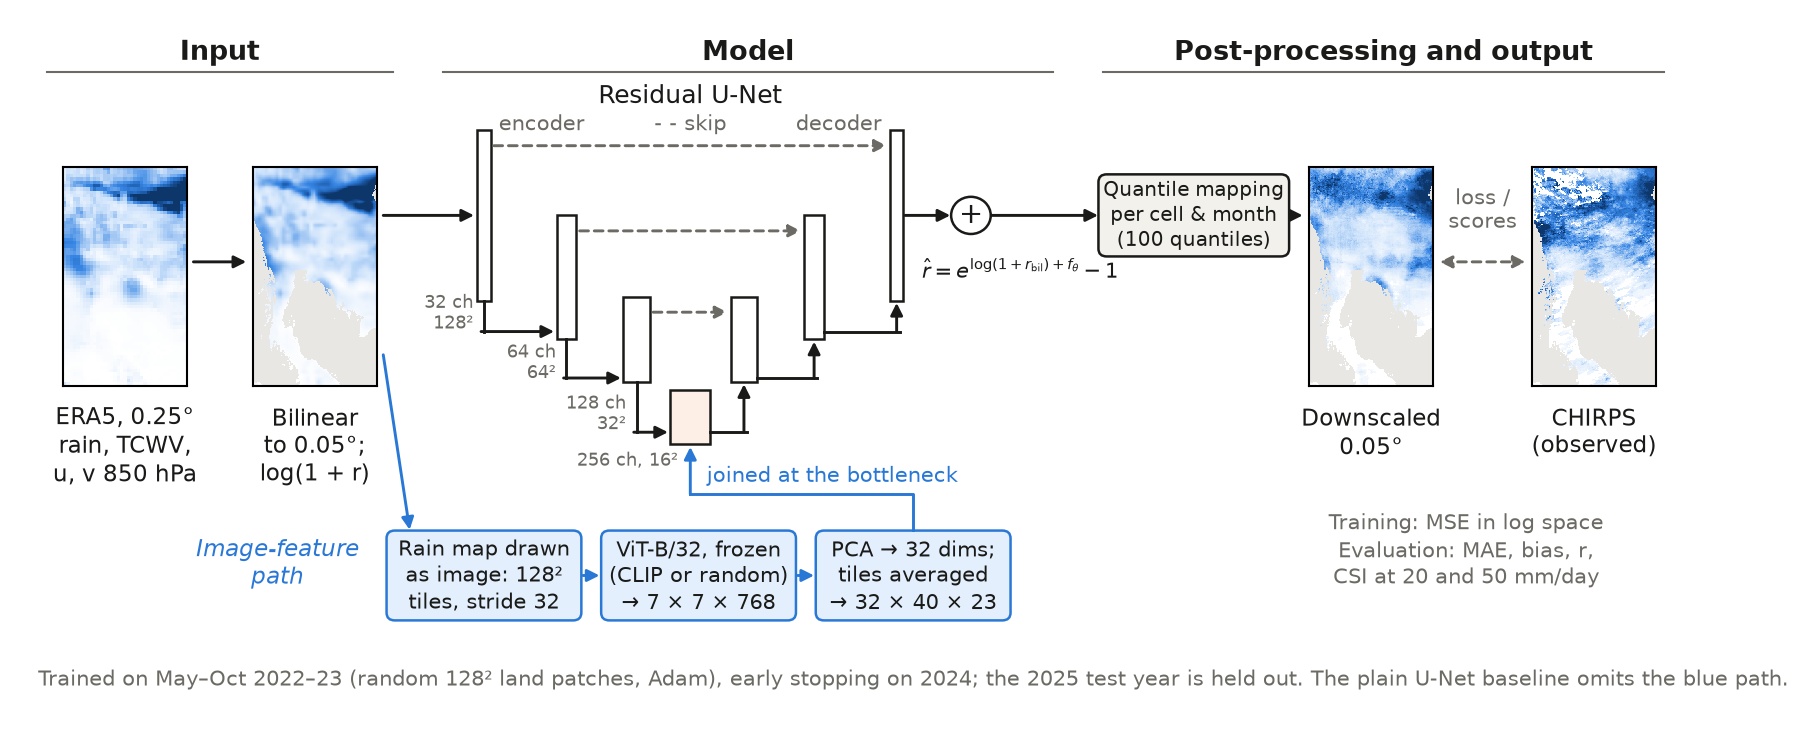
\includegraphics[width=\textwidth]{figures/workflow_medium.png}
  \caption{Overview of the proposed model. ERA5 fields are interpolated to
  the 0.05\textdegree{} CHIRPS grid and passed through a residual U-Net
  (dashed: skip connections). In the image-feature path (blue), the
  interpolated rain map is drawn as image tiles, encoded by a frozen
  ViT-B/32 with CLIP or random weights, and reduced by PCA to 32 maps that
  join the bottleneck. The predicted log residual is added to bilinear
  rain, and quantile mapping corrects the distribution. The output is
  trained and evaluated against CHIRPS. The maps show 22~September~2024.
  The plain U-Net baseline omits the blue path.}
  \Description{Flow diagram in three stages. Input: ERA5 and bilinear rain
  maps. Model: a U-shaped network with three encoder and three decoder
  levels, skip connections, and a bottleneck that receives feature maps
  from a blue path of three boxes (image tiles, frozen ViT-B/32, PCA).
  Output: residual addition, quantile mapping, the downscaled map, compared
  with the CHIRPS map.}
  \label{fig:workflow}
\end{figure*}

Figure~\ref{fig:workflow} shows the proposed model from input to output.
The four ERA5 fields are interpolated to the CHIRPS grid (input stage) and
passed through a three-level residual U-Net, whose skip connections (dashed)
carry fine detail from the encoder to the decoder. The image-feature path
(blue) is the only addition to the plain U-Net: it turns the interpolated
rain map into 32 feature maps that enter at the bottleneck, where the
network has the widest view of the field. The U-Net output is a correction
in log space, so it is added to bilinear rain, and quantile mapping then
adjusts the distribution of each land cell. The following paragraphs
describe each component.

\textbf{Baselines.} \emph{Bilinear} interpolation of ERA5 rain.
\emph{Quantile mapping} (QM) maps, for each land cell and calendar month,
100 quantiles of a base model's 2022--2023 output onto those of CHIRPS;
above the largest training value, the top correction is added. We apply QM
both to bilinear rain and on top of each U-Net, fitted on that U-Net's own
training-year predictions.

\textbf{U-Net.} A three-level U-Net~\cite{ronneberger2015unet} (base
width 32, 1.93\,M parameters) predicts a residual in log space,
$\hat r = \exp\!\big(\log(1+r_{\mathrm{bil}}) + f_\theta(x)\big) - 1$, so
the network only learns what bilinear interpolation gets wrong. It is
trained with a mean squared error on land cells, on random
$128\times128$ patches (Adam~\cite{kingma2015adam}, learning rate
$10^{-3}$, batch 8), with early
stopping (patience 5, at most 40 epochs) on the 2024 validation loss.

\textbf{Count loss.} As a non-CLIP region-level loss, we compare the share
of land cells above 20 and 50\,mm in the prediction and the observation,
using a sigmoid threshold (width 2\,mm) so the share is differentiable.
Shares are computed for the full patch and its centred half and quarter,
and the mean absolute gap is added with weight $\lambda=10$.

\textbf{CLIP loss (MRA).} We adapt the MRA loss of
Clip4Rain~\cite{li2026clip4rain}; its multi-scale consistency term
targets the temporal encoder of a nowcasting network and has no
counterpart in our single-step U-Net, so we omit it. Rain
maps are drawn as RGB images with a fixed seven-step blue colour map
(0--100\,mm, sea in grey), resized to $224\times224$ and passed through
frozen OpenAI CLIP with a ViT-B/32 image
encoder~\cite{radford2021clip,dosovitskiy2021vit,cherti2023openclip}.
Each observed crop (full, half, quarter) is described as ``There is
\{no, little, some, a lot of\} heavy rain in the image.'', depending on
whether 0\%, up to 5\%, up to 20\% or more than 20\% of its land exceeds
20\,mm. The \emph{text} loss penalises
$|\,s(\hat y, t) - s(y, t)\,|$, where $s$ is the cosine similarity between
an image and the sentence $t$ of the observed crop ($\lambda = 20$). The
\emph{image} ablation uses $1 - s(\hat y, y)$ between the two images
instead ($\lambda=3$). Unlike Clip4Rain, which counts rain pixels in the
prompt and passes the text embeddings through a learnable MLP, we use fixed
sentences about heavy rain, the quantity we want to improve, so that the
loss depends on CLIP alone. CLIP is used only during training.

\textbf{CLIP patch features as input.} The CLIP loss only judges outputs.
We also test CLIP as a description of the \emph{input}. The ERA5 rain map
(bilinear, on the fine grid) is cut into overlapping $128\times128$ tiles
(stride 32; 21 tiles per day), drawn with the same colour map, and encoded
by frozen CLIP. Instead of the single image vector, we keep the $7\times7$
grid of patch tokens (768 values each), which preserves spatial layout.
PCA, fitted on tokens from every sixth training day, reduces each token to
32 standardised components. Each tile's grid is interpolated to
$16\times16$, the bottleneck resolution of a $128\times128$ patch, and
overlapping tiles are averaged into one $40\times23$ map per day. The 32
maps are concatenated to the bottleneck input of the U-Net (2.00\,M
parameters). Because every feature is computed from a tile of the same
size, training patches and whole-field prediction see features at the same
scale, and only ERA5 is used, so the method applies to any day. Training
patch corners are restricted to multiples of 8 so that the feature maps can
be cut out exactly.

\textbf{Random-weight control.} The same pipeline, but the ViT-B/32 has
random weights (fixed seed) instead of CLIP's pretrained weights. Tiling,
colour map, PCA and U-Net are identical. Any gain shared by both variants
comes from the extra input path, not from pretraining. Random features are
a known strong baseline~\cite{rahimi2007random}, and transfer studies in
other domains found that pretrained weights often help less than
assumed~\cite{raghu2019transfusion}.

\textbf{Seeds.} The plain U-Net, the CLIP-input U-Net and the control are
each trained with three seeds (initialisation and patch sampling); we
report the mean and the range. The loss variants were run once.

%% ---------------------------------------------------------------------
\section{Can CLIP Read Rain Maps?}

Before using CLIP, we asked whether it can tell light rain from heavy
rain on our maps. Table~\ref{tab:diag} summarises four tests: part~(a)
asks whether OpenAI CLIP can read rain amounts from CHIRPS maps, and
part~(b) whether image embeddings of the ERA5 input add information
beyond simple statistics, for three encoders.

\textbf{Zero-shot sentences (Table~\ref{tab:diag}a, first row).} For 300 random $128\times128$ CHIRPS crops
from 2024 (at least half land), CLIP chose the correct sentence for 22\%,
below chance (25\%) and well below always predicting the most common class
(42\%).

\textbf{Sensitivity to intensity (Table~\ref{tab:diag}a, third row).} When the rain of 40 wet crops was
multiplied by 0, 1 and 4, the mean similarity to the ``a lot of'' sentence
was 0.219, 0.270 and 0.278: CLIP reacts to rain being present, but barely
to rain becoming much heavier. Part of this is caused by the colour map,
which saturates at 100\,mm.

\textbf{Linear information (Table~\ref{tab:diag}a, second row).} A nearest-centroid classifier on CLIP image
features, fitted on 300 crops from 2022--2023, reached 47\% on 2024 (most
common class: 42\%).

\textbf{Features of the ERA5 input (Table~\ref{tab:diag}b).} For the input variant, the relevant
question is whether image features of the \emph{ERA5} map add information
beyond simple statistics. On 1000 training and 500 validation crops, we
predicted the share of land with at least 20\,mm in CHIRPS with ridge
regression. Eighteen ERA5 statistics (mean, standard deviation, 90th
percentile and maximum of each input, plus the share of bilinear rain above
10 and 20\,mm) reached RMSE 0.0824 ($R^2 = 0.49$). Adding 16 PCA
components of the rain-map embedding lowered the RMSE by only 0.0015 for
CLIP (95\% bootstrap interval~\cite{efron1993bootstrap} $-0.0001$ to
$+0.0031$), 0.0008 for
RemoteCLIP and 0.0006 for SigLIP; adding embeddings of all four inputs gave
no further gain. Embeddings alone did worse than the statistics.

Taken together, Table~\ref{tab:diag} shows that CLIP registers whether a
map contains rain but not how much, and that neither CLIP nor its
remote-sensing (RemoteCLIP) or newer (SigLIP) counterparts add significant
information about heavy rain beyond 18 simple ERA5 statistics. A CLIP-based
loss therefore has little to reward, and any benefit of CLIP features as an
input must come from somewhere other than an understanding of rain
intensity.

\begin{table}
  \caption{Diagnostics of frozen image encoders on rain maps (2024 crops).}
  \label{tab:diag}
  \footnotesize
  \setlength{\tabcolsep}{4pt}
  \begin{tabular}{@{}p{0.38\columnwidth}ccc@{}}
    \toprule
    \multicolumn{4}{@{}l}{\textbf{(a) OpenAI CLIP on CHIRPS rain maps}} \\
    \midrule
    Correct sentence (zero-shot)
      & \multicolumn{3}{c}{22\% \ (chance 25\%, majority 42\%)} \\
    Nearest-centroid classifier
      & \multicolumn{3}{c}{47\% \ (majority 42\%)} \\
    Similarity to ``a lot of'', rain $\times0$\,/\,$\times1$\,/\,$\times4$
      & \multicolumn{3}{c}{0.219\,/\,0.270\,/\,0.278} \\
    \midrule
    \multicolumn{4}{@{}l}{\textbf{(b) RMSE of heavy-rain share from ERA5 (lower is better)}} \\
    \midrule
    Features & CLIP & RemoteCLIP & SigLIP \\
    \midrule
    ERA5 statistics only & \multicolumn{3}{c}{0.0824} \\
    Statistics + embedding & 0.0810 & 0.0816 & 0.0818 \\
    Embedding only & 0.0874 & 0.0883 & 0.0883 \\
    \bottomrule
  \end{tabular}
\end{table}

Finally, we checked that the random control is not handicapped. On 12
validation days, 62\% of the variance of the random-network features
varied from day to day (CLIP: 33\%), and the best single component
correlated with bottleneck-averaged ERA5 rain at 0.70 (CLIP: 0.33). The
random network passes the rain map through more directly, while much of
CLIP's feature variance encodes fixed patterns such as the coastline.

%% ---------------------------------------------------------------------
\section{Results}

Table~\ref{tab:main} lists the 2024 validation scores. Its upper block
contains the baselines and the U-Nets as trained; the lower block the
U-Nets with QM applied on top. Models marked $\dagger$ were trained with
three seeds, and the CSI$_{20}$ column in brackets gives their range, which
shows whether a difference between models exceeds the variation between
runs. Figure~\ref{fig:maps} shows the models on the wettest validation day,
and Figure~\ref{fig:exceed} the distribution of daily amounts over the
whole season.

\begin{figure*}
  \centering
  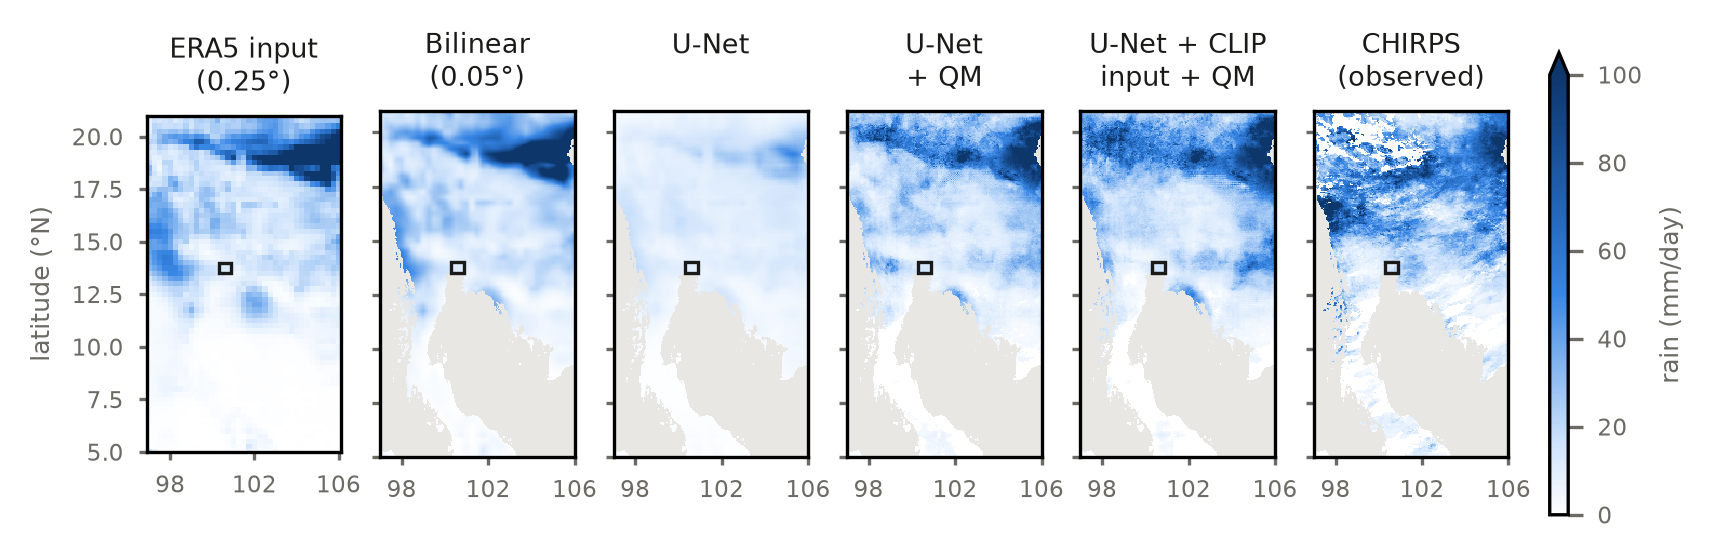
\includegraphics[width=\textwidth]{figures/maps_paper.png}
  \caption{Daily rain on 22 September 2024, the validation day with the
  largest share of land above 50\,mm (seed-0 models, same colour scale,
  land only; the box marks Bangkok). Bilinear interpolation keeps ERA5's
  blocky pattern; the U-Net trained with mean squared error is smooth and
  far too dry. QM restores realistic amounts in the north, and the two QM
  maps, with and without CLIP input, look almost the same. No model
  reproduces the heavy rain along the western border or the small-scale
  structure of CHIRPS.}
  \Description{Six maps of Thailand: ERA5 input, bilinear, U-Net, U-Net
  with quantile mapping, CLIP-input U-Net with quantile mapping, and CHIRPS.
  The plain U-Net is nearly white; the two quantile-mapped maps look alike
  and show heavy rain in the north, as CHIRPS does, but not along the
  western border.}
  \label{fig:maps}
\end{figure*}

\begin{table*}
  \caption{Validation scores on 2024 (183 days, land cells). Models
  marked $\dagger$ are the mean over three seeds; the range (min--max) of
  CSI$_{20}$ is given in brackets. Best value in each column in bold
  (bias: closest to zero).}
  \label{tab:main}
  \small
  \begin{tabular}{lrrrrrcrr}
    \toprule
    & \multicolumn{6}{c}{Thailand} & \multicolumn{2}{c}{Bangkok} \\
    \cmidrule(lr){2-7}\cmidrule(lr){8-9}
    Model & MAE & Bias & Corr & CSI$_{20}$ & CSI$_{50}$ & CSI$_{20}$ range
      & Corr & CSI$_{20}$ \\
    \midrule
    Bilinear            & 7.90 & $\mathbf{-0.26}$ & 0.440 & 0.222 & 0.098 & -- & 0.378 & 0.129 \\
    QM                  & 8.87 & $+0.49$ & 0.437 & 0.254 & 0.128 & -- & 0.309 & 0.129 \\
    U-Net$^\dagger$     & 7.09 & $-4.27$ & 0.480 & 0.047 & 0.003 & [0.042, 0.057] & 0.440 & 0.009 \\
    U-Net + count loss  & 7.43 & $-2.35$ & 0.422 & 0.178 & 0.082 & -- & 0.381 & 0.109 \\
    U-Net + CLIP loss (text)  & 7.24 & $-4.05$ & 0.409 & 0.051 & 0.012 & -- & 0.416 & 0.004 \\
    U-Net + CLIP loss (image) & 7.12 & $-4.24$ & 0.464 & 0.070 & 0.018 & -- & 0.411 & 0.005 \\
    U-Net + CLIP input$^\dagger$  & 7.03 & $-4.37$ & \textbf{0.496} & 0.055 & 0.014 & [0.025, 0.108] & \textbf{0.479} & 0.012 \\
    U-Net + random input$^\dagger$ & \textbf{6.94} & $-3.98$ & 0.484 & 0.072 & 0.001 & [0.061, 0.095] & \textbf{0.479} & 0.001 \\
    \midrule
    U-Net + QM$^\dagger$              & 8.50 & $+0.85$ & 0.476 & 0.275 & \textbf{0.144} & [0.271, 0.278] & 0.360 & 0.124 \\
    U-Net + CLIP input + QM$^\dagger$ & 8.35 & $+0.83$ & 0.488 & \textbf{0.282} & 0.142 & [0.280, 0.284] & 0.402 & \textbf{0.133} \\
    U-Net + random input + QM$^\dagger$ & 8.28 & $+0.65$ & 0.474 & 0.280 & 0.134 & [0.278, 0.282] & 0.407 & 0.121 \\
    \bottomrule
  \end{tabular}
\end{table*}

\begin{figure}
  \centering
  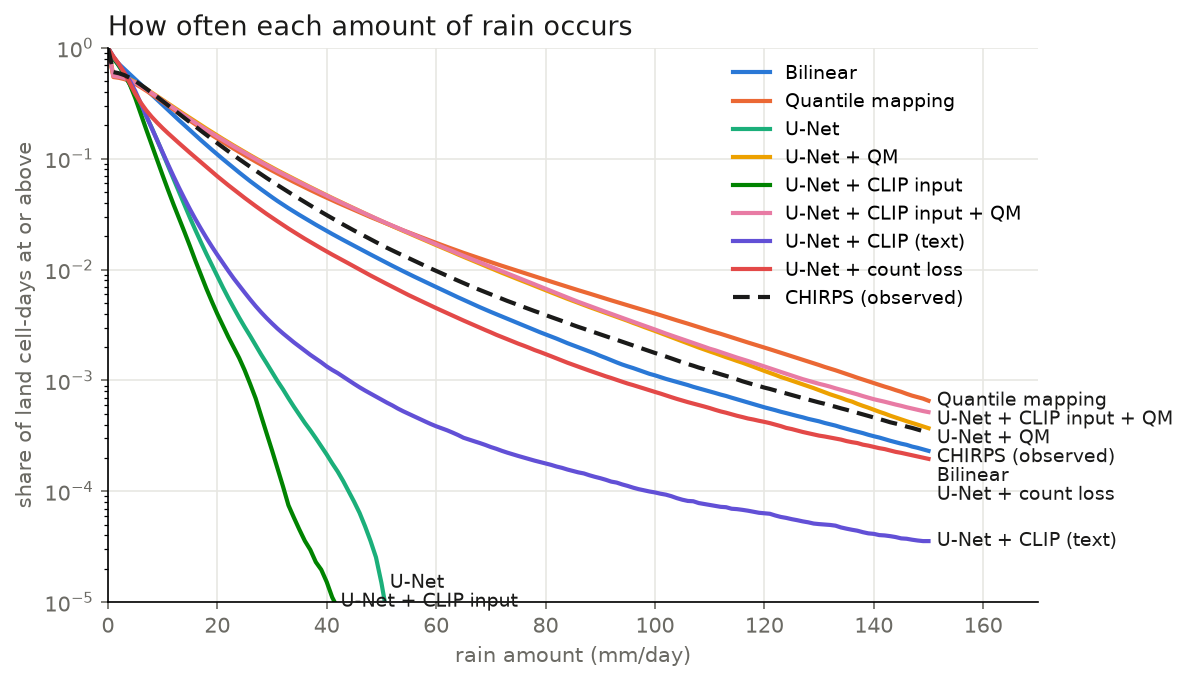
\includegraphics[width=\columnwidth]{figures/exceedance_val.png}
  \caption{Share of land cell-days at or above each daily amount in 2024
  (seed-0 runs, log scale). U-Nets trained with mean squared error alone,
  with or without CLIP input, fall far below CHIRPS (dashed) beyond
  20\,mm. The CLIP text loss adds a thin tail of heavy values, still more
  than ten times too rare; the count loss lies just below CHIRPS; and the
  QM models lie slightly above it. The image-only CLIP loss and the random
  control are omitted for readability.}
  \Description{Exceedance curves on a log scale for each model and for
  CHIRPS. Plain and CLIP-input U-Nets drop below one in ten thousand
  before 50 mm per day, while quantile-mapped models follow the observed
  curve.}
  \label{fig:exceed}
\end{figure}

\textbf{CLIP losses do not fix underestimation.} In the upper block of
Table~\ref{tab:main}, all U-Nets trained with mean squared error have the
lowest MAE but a strong dry bias ($-4.3$\,mm/day) and almost no skill above
20\,mm (CSI$_{20}$ 0.05, CSI$_{50}$ near 0). Figure~\ref{fig:exceed} shows
why: their predicted amounts almost never exceed 40--50\,mm, while CHIRPS
has 1\% of land cell-days above 60\,mm. The CLIP text and image losses
change this very little (CSI$_{20}$ 0.05--0.07); the text loss produces
some heavy values, but more than ten times too rarely. The simple count
loss, which compares heavy-rain shares directly, is far more effective
(bias $-2.35$, CSI$_{20}$ 0.18), and its curve lies just below CHIRPS. QM
on top of the U-Net is best for heavy rain (lower block; CSI$_{20}$ 0.275,
CSI$_{50}$ 0.144); its curve lies slightly above CHIRPS, matching its small
wet bias ($+0.85$), and its MAE is higher, the usual trade-off once heavy
rain is predicted with uncertain location.

\textbf{Spatial patterns.} Figure~\ref{fig:maps} shows the same behaviour
on 22 September 2024. Bilinear interpolation keeps the blocky 0.25\textdegree{}
pattern of ERA5; the plain U-Net smooths it into an almost dry field; QM
restores heavy rain in the north, where CHIRPS has it. All models,
however, miss the band of heavy rain along the western border and the
small-scale structure of CHIRPS, which ERA5 does not resolve. The two QM
maps, with and without CLIP input, are hard to tell apart on a single day,
in line with the small differences in Table~\ref{tab:main}.

\textbf{CLIP input improves placement.} Without QM (upper block of
Table~\ref{tab:main}), CLIP input gives the
highest correlation in Thailand (0.496 vs.\ 0.480), but it does not raise
heavy-rain skill, and its validation loss is lower than that of the plain
U-Net for all three seeds (1.268 vs.\ 1.308 on average). With QM, the
better placement carries through: CSI$_{20}$ rises from 0.275 to 0.282,
and the three CLIP-input runs (0.280--0.284) all beat the three plain runs
(0.271--0.278). Correlation (0.488 vs.\ 0.476) and MAE (8.35 vs.\ 8.50)
also improve. There is no gain at 50\,mm, and in Bangkok no model detects
any of the 37 observed cell-days above 50\,mm.

\textbf{The random control recovers most of the gain.} The last row of
Table~\ref{tab:main} is the decisive comparison. With random weights
instead of CLIP, the U-Net with QM reaches CSI$_{20}$ 0.280
(0.278--0.282), which overlaps with CLIP (0.280--0.284), and it has a
lower MAE and bias. Its validation loss is also as low as CLIP's (1.260
vs.\ 1.268). About 70\% of the CSI$_{20}$ gain over U-Net with QM
($+0.005$ of $+0.007$) is therefore obtained without pretraining. The only
advantage specific to CLIP is a slightly higher correlation in Thailand
after QM (0.488 vs.\ 0.474), with seed ranges that nearly touch
(0.480--0.494 vs.\ 0.463--0.483). In Bangkok, both feature variants raise
correlation over U-Net with QM by a similar amount (0.40--0.41 vs.\ 0.36).

\begin{table*}
  \caption{Test scores on 2025 (183 days, land cells), computed once with
  the final models. Notation as in Table~\ref{tab:main}.}
  \label{tab:test}
  \small
  \begin{tabular}{lrrrrrcrr}
    \toprule
    & \multicolumn{6}{c}{Thailand} & \multicolumn{2}{c}{Bangkok} \\
    \cmidrule(lr){2-7}\cmidrule(lr){8-9}
    Model & MAE & Bias & Corr & CSI$_{20}$ & CSI$_{50}$ & CSI$_{20}$ range
      & Corr & CSI$_{20}$ \\
    \midrule
    Bilinear          & 8.24 & $-0.47$ & 0.418 & 0.209 & 0.107 & -- & 0.530 & 0.178 \\
    QM                & 9.02 & $+0.23$ & 0.432 & 0.245 & 0.150 & -- & 0.524 & 0.171 \\
    U-Net$^\dagger$   & \textbf{7.50} & $-4.63$ & 0.463 & 0.042 & 0.001 & [0.032, 0.051] & \textbf{0.553} & 0.040 \\
    \midrule
    U-Net + QM$^\dagger$                & 8.45 & $\mathbf{-0.02}$ & 0.467 & 0.263 & 0.157 & [0.253, 0.271] & 0.527 & 0.177 \\
    U-Net + CLIP input + QM$^\dagger$   & 8.22 & $-0.21$ & 0.480 & 0.271 & \textbf{0.159} & [0.268, 0.275] & 0.509 & \textbf{0.180} \\
    U-Net + random input + QM$^\dagger$ & 8.25 & $-0.28$ & \textbf{0.485} & \textbf{0.273} & \textbf{0.159} & [0.270, 0.278] & 0.519 & 0.160 \\
    \bottomrule
  \end{tabular}
\end{table*}

\textbf{The test year confirms the result.} Table~\ref{tab:test} gives the
scores on 2025, which played no part in training, early stopping or any
design decision. All scores are slightly lower than in 2024, but the
pattern is the same. Without QM, the U-Net again has the lowest MAE and
almost no heavy-rain skill; with QM, the extra input path raises
CSI$_{20}$ from 0.263 to 0.271 with CLIP features and to 0.273 with
random features, and it raises correlation from 0.467 to 0.480 and 0.485.
The random control now matches or exceeds CLIP on every Thailand score,
so the small correlation advantage of CLIP seen in 2024 does not
generalise. The gain over U-Net with QM is also less clear-cut than in
2024: the best plain run (0.271) lies within the CLIP-input range
(0.268--0.275). At 50\,mm all three QM models are equal (0.157--0.159),
and in Bangkok, where a single season holds few heavy-rain days, none of
the feature variants improves on U-Net with QM.

%% ---------------------------------------------------------------------
\section{Discussion and Limitations}

The diagnostics and the control tell a consistent story. CLIP was trained
on photographs and their captions; a colour-coded rain map is far from that
domain, and CLIP neither ranks rain intensity nor links our sentences to
the maps. A loss built on its similarities therefore gives the U-Net
little to learn from. As an input, a coarse second view of the rain map at
the bottleneck helps the network place rain, plausibly because each
feature summarises a whole $128\times128$ tile, wider context than the
bottleneck sees otherwise, but this works equally well with random
weights. Heavy-rain skill, finally, appears limited by the training
objective rather than the inputs: every model trained with mean squared
error smooths the peaks, and only distribution corrections (QM) or losses
on heavy-rain shares recover them.

The study has clear limits. It covers one region, one season and two
training years, and a single test season. The validation year was also
used for early stopping, so its absolute scores are optimistic for all
models alike; the 2025 test scores are unbiased but come from one season,
and the differences between the three QM models are of the same size as
the spread between seeds. The CLIP losses were run
with one seed and one weight each, and we tried one prompt template and one
colour map, which saturates at 100\,mm. CHIRPS is itself an estimate from
satellites and gauges, at about 5\,km rather than the 1--3\,km often
needed. We did not fine-tune CLIP on rain maps, nor test newer encoders
with stronger dense features such as SigLIP~2~\cite{tschannen2025siglip2},
which could change the picture.

%% ---------------------------------------------------------------------
\section{Conclusion}

Frozen CLIP, used as a loss or as an input, did not improve heavy-rain
downscaling over Thailand beyond what simpler tools achieve. Its features
as a U-Net input gave a small improvement after quantile mapping, but a
network with random weights reproduced most of it on the validation year
and all of it on the held-out test year. Claims
that vision--language pretraining helps geospatial downscaling should
therefore be checked against such random-weight controls. Promising next
steps are renderings that preserve heavy-rain intensity, fine-tuning on
rain maps, text that carries information absent from the inputs, such as
issued weather forecasts, and generative models that address the
smoothing of pixel-wise losses directly~\cite{mardani2025corrdiff}.

\begin{acks}
This work was supported by the Chula-LINK Scholarship of Chulalongkorn
University. We thank the European Centre for
Medium-Range Weather Forecasts (ECMWF) and the Copernicus Climate Change
Service for providing ERA5, and the Climate Hazards Center, University of
California, Santa Barbara, for providing CHIRPS. ERA5 data were obtained
from the Copernicus Climate Data Store. The views expressed are those of
the authors and do not necessarily reflect those of the funding
institution.
\end{acks}

\bibliographystyle{ACM-Reference-Format}
\bibliography{refs}

\end{document}
\endinput
